
\documentclass[11pt,a4paper,oneside]{article}
\usepackage[dutch]{babel}
\usepackage{amsmath}
\usepackage{graphicx}
\usepackage{tikz}
\usepackage{fancyhdr}
\usepackage{dsfont}
\usepackage[official]{eurosym}
\usepackage{parskip}
\usepackage{epstopdf}
\usepackage{listings}
\usepackage{color}
\definecolor{lichtgrijs}{gray}{0.95}
\usepackage{cite}
\usepackage[nottoc]{tocbibind}
\usepackage[T1]{fontenc}
\usepackage[light,math]{iwona}
\usepackage{pgfplots}
\pgfplotsset{compat=newest}
\usepackage{subfig}
\usepackage{textcomp}
\usetikzlibrary{arrows,automata}
\usepackage{float}
\usepackage{longtable}
\usepackage{titling,enumitem}
\usepackage{a4wide}
\usepackage{amssymb}
\usepackage{rotating}
\usepackage{listings}
\usepackage[top=1.1in, bottom=1.2in, left=1.1in, right=1.1in]{geometry}
\usepackage{array}
\usepackage{titling}
\usepackage{blindtext}
\usepackage{chngpage}
\usepackage{calc}
\definecolor{lightgray}{gray}{0.8}
\newcolumntype{L}{>{\raggedleft}p{0.50\textwidth}}
\newcolumntype{R}{p{0.8\textwidth}}
\newcommand\VRule{\color{lightgray}\vrule width 0.5pt}
\usepackage{color, colortbl}
\definecolor{Gray}{gray}{0.9}
\definecolor{dkgreen}{rgb}{0,0.6,0}
\definecolor{gray}{rgb}{0.5,0.5,0.5}
\definecolor{mauve}{rgb}{0.58,0,0.82}
\definecolor{ugentblue}{rgb}{0.05,0.18,0.37}
\usepackage{import}
\usepackage[T1]{fontenc}
\begin{document}

\newgeometry{top=0.8cm, right=1.70cm, left=1.7cm}
\begin{titlepage}

\thispagestyle{fancy}
\fancyhf{}
\fancyfoot[L]{}
\begin{figure}[!ht]
  \begin{adjustwidth}{-\oddsidemargin-1in}{-\rightmargin}
    \centering
    
\includegraphics[width=\paperwidth]{img/banner}
  \end{adjustwidth}
\end{figure}
\vspace{-0.2em}
\begin{center}
\vspace{5cm}
\Huge \textbf{Vakoverschrijdend Project: team Edran\\ Gebruikershandleiding}\\
\vspace{6.0cm}
\large
\begin{tabular}{L! {} R}
& {\LARGE\bf Team Edran} \\
& \\
& {\bf Steven De Blieck} \\
& {\bf Laurens De Graeve} \\
& {\bf Bart Middag} \\
& {\bf Wouter Pinnoo} \\
& {\bf Robin Praet} \\
& {\bf Stijn Seghers} \\
& {\bf Wouter Termont} \\
& {\bf Gilles Vandewiele} \\
\end{tabular}
\end{center}
\end{titlepage}
\restoregeometry
\newpage

\fancyheadoffset[RO,LE]{0in}
\fancypagestyle{plain}{
\fancyhead[L]{Gebruikershandleiding}
\fancyhead[R]{Team Edran}
\fancyfoot[L]{}
\fancyfoot[R]{\thepage}}

\fancyhead[L]{Gebruikershandleiding}
\fancyhead[R]{Team Edran}
\fancyfoot[L]{}
\fancyfoot[C]{\thepage}
\pagestyle{fancy}
\tableofcontents
\newpage

\section{Eerste keer op onze website}
\subsection{Menubalk}

\includegraphics[scale=0.35]{img/menubalk} \\\\
Als we in dit document verwijzen naar de menubalk dan bedoelen we telkens de groene balk bovenaan elke pagina. Deze bevat - bij het eerste bezoek aan de website - het logo van D\'egage, \textit{Registreren} en \textit{Aanmelden}. Op \textit{Registreren} en \textit{Aanmelden} komen we later terug, maar het logo van D\'egage doet hier dienst als de homeknop. Indien u hier op drukt, komt u telkens terecht bij de beginpagina. Deze zal uiteraard anders zijn afhankelijk of u al dan niet bent ingelogd en afhankelijk van welke functie u zal vervullen.
\subsection{Welkom}
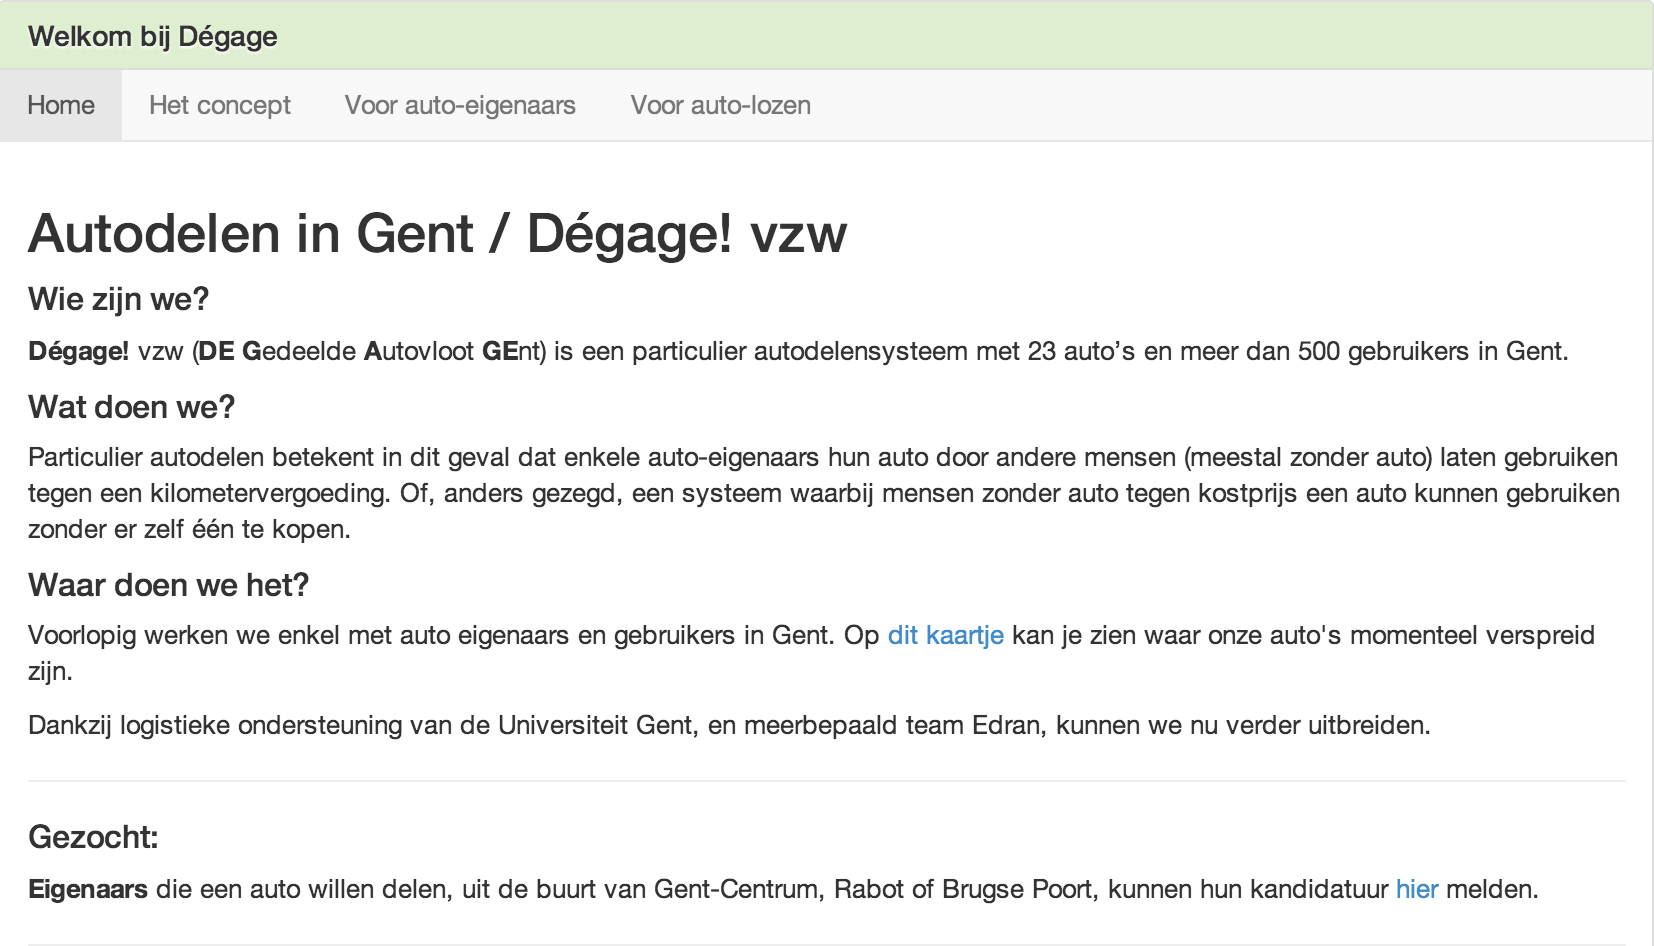
\includegraphics[scale=0.60]{img/home}
\\
Als u voor de eerste keer onze website bezoekt, wordt er uitgelegd wat D\'egage is, wat het doet en waar het actief is. Dit om een beter beeld te schetsen van de vereniging. Indien u al een account hebt, is het mogelijk om in te loggen via de menubalk bovenaan. In het andere geval is het vereist eerst de registratieprocedure te voltooien. Dit kan eenvoudig door op de link \textit{hier} te klikken, welke te vinden is onder de titel \textbf{Gezocht}. Indien u alsnog twijfels heeft, raden wij u aan om de tabbladen \textit{Het concept, Voor auto-eigenaars, Voor auto-lozen} te lezen. Het is namelijk belangrijk te weten of u enkel een auto wilt lenen of ook uw eigen auto ter beschikking wilt stellen. En vooraleer u ten volle kan genieten van de website, is het natuurlijk handig het volledige concept te weten.\\\\

\section{Aanmelden}
In het geval dat u al in het bezit bent van een account, is het mogelijk om via deze weg in te loggen. 
Kan u uw wachtwoord niet meer voor de geest halen? Geen nood, via \textit{Wachtwoord vergeten?} is het mogelijk uw wachtwoord te resetten.\\
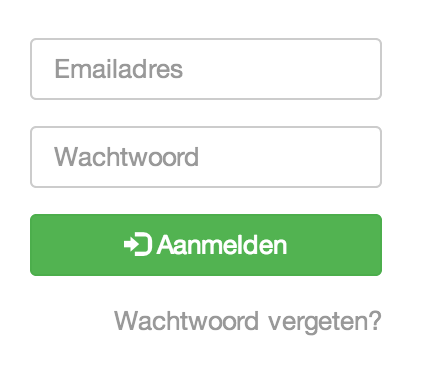
\includegraphics[scale=0.75]{img/login}

\subsection{Wachtwoord vergeten}
\subsubsection{Emailadres niet vergeten}
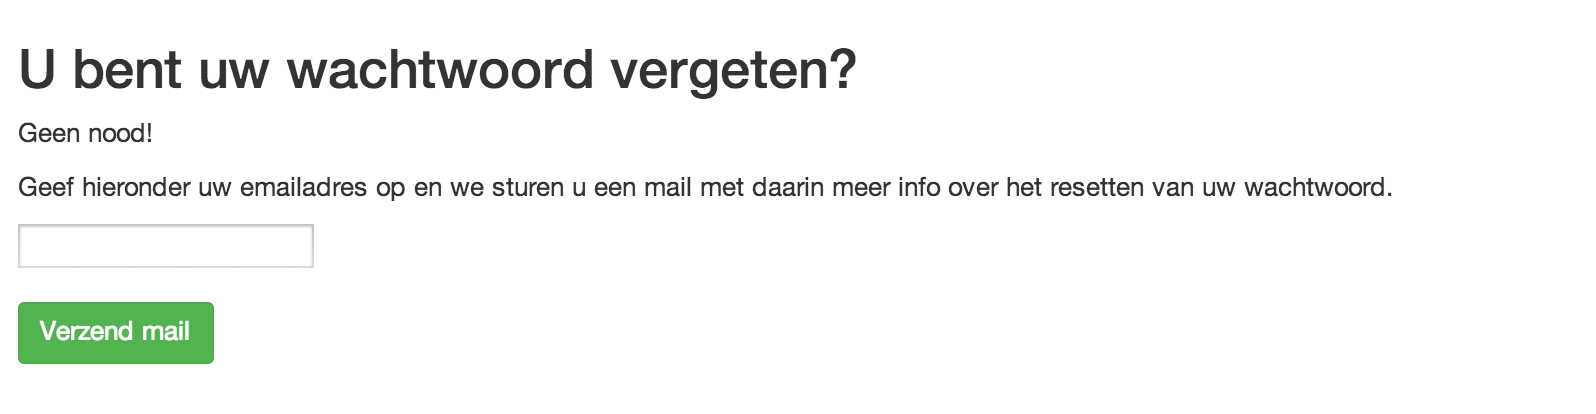
\includegraphics[scale=0.5]{img/emailnietvergeten} \\
In dit geval zal uw wachtwoord gereset worden. Daarvoor is het nodig uw emailadres in de witte balk in te vullen en op \textit{Verzend mail} te drukken. Daarna raden wij u aan om uw emails te bekijken en daar  de stappen verder te volgen.
\subsubsection{Emailadres ook vergeten}
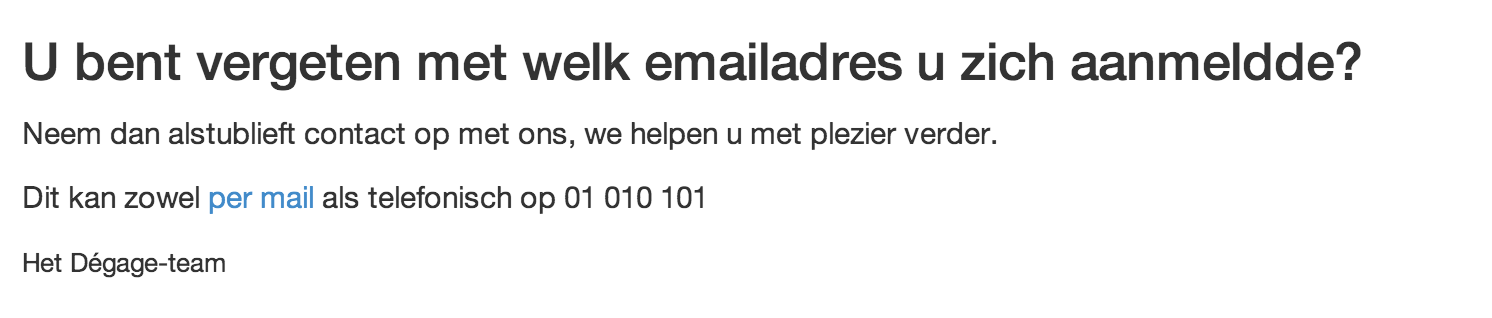
\includegraphics[scale=0.5]{img/emailookvergeten} \\\\
In dit geval is het uiteraard moeilijk u een email te sturen. We raden u in dit geval aan om ons ofwel een mailtje sturen naar edran.vopro@gmail.com ofwel ons eens te bellen, waar we het probleem dan met plezier verder zullen oplossen.


\section{Registreren}

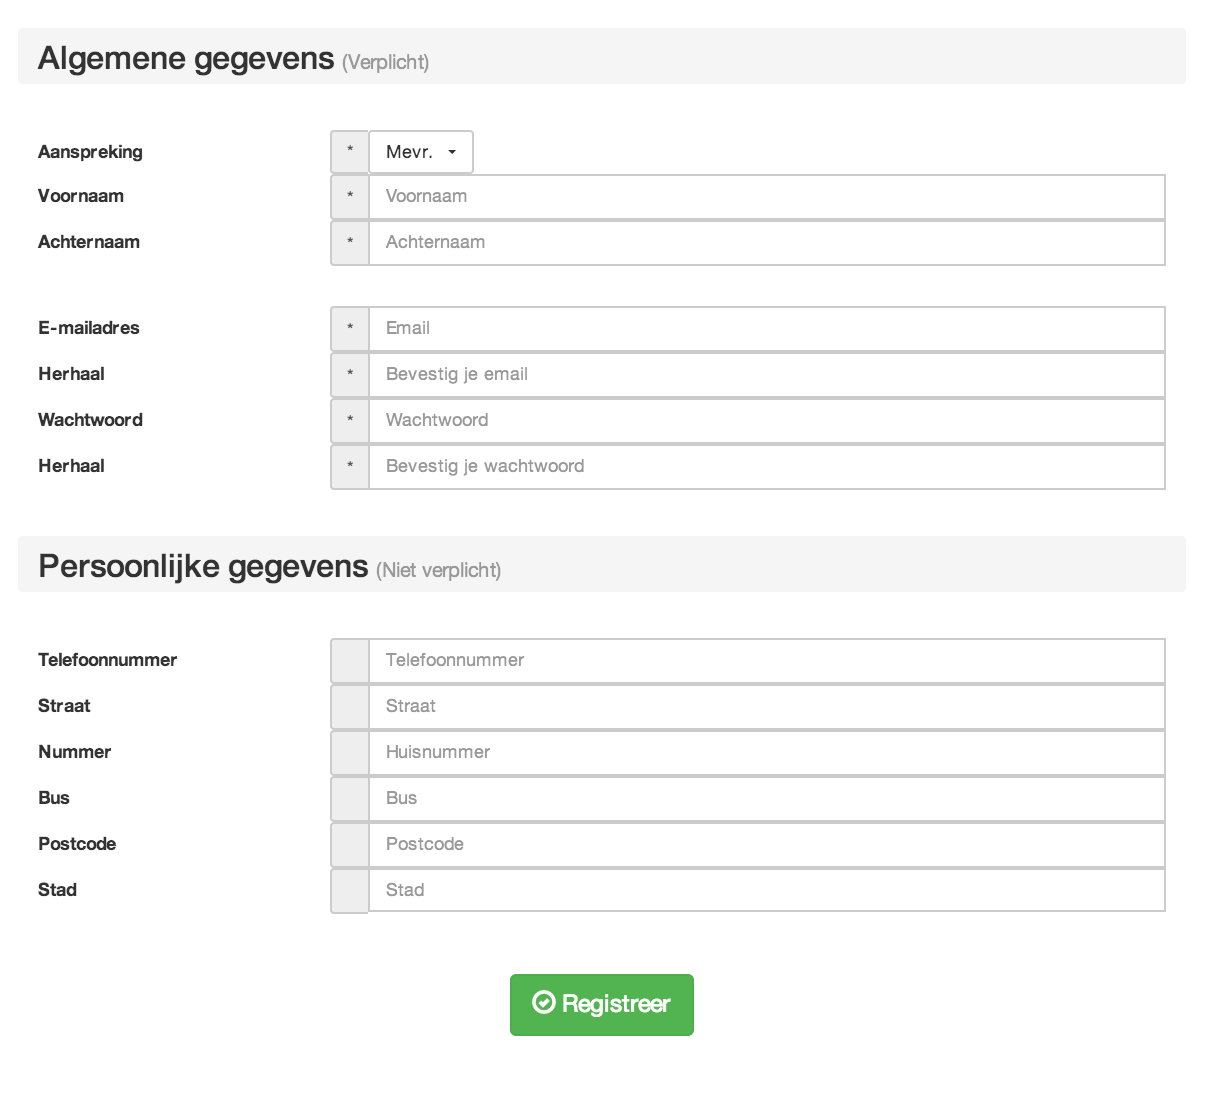
\includegraphics[scale=0.6]{img/registreren99} \\\\

Indien u nog geen lid bent van D\'egage en dit wel graag zou worden, is het noodzakelijk u eerst en vooral te registreren op de site via het invullen van allerlei gegevens. De velden met een sterretje zijn verplicht, de andere optioneel. De registratieprocedure is opgedeeld in 2 formulieren. De \textbf{Algemene gegevens} zijn verplicht en moeten bijgevolg ingevuld worden alvorens u de registratie succesvol kan be\"eindigen. De \textbf{Persoonlijke gegevens} zijn allemaal optioneel, maar wij raden u aan om deze toch in te vullen. In dit geval hebben wij meer informatie over u en kunnen wij u bijvoorbeeld opbellen bij uiterst urgente zaken. Het spreekt voor zich dat wij geen misbruik zullen maken van deze gegevens. Na het registreren ontvangt u - als alles goed gaat tenminste- een mailtje met de melding dat uw registratie geslaagd is. Nu is het enkel nog nodig om uw emailadres te verifi\"eren door op de link in de mail te drukken. Vervolgens is het dus mogelijk om u in te loggen, zoals daarnet beschreven.

\section{Autolener of auto-eigenaar?}
Nu is het nodig om een keuze te maken. Ofwel stelt u uw eigen auto ter beschikking van D\'egage ofwel leent u enkel auto's.
\subsection{Autolener}
Indien u enkel auto's wilt lenen, is de volgende stap u in te schrijven voor een infosessie. Dit kan door op \textit{Infosessies} te drukken in de menubalk. \\\\


\includegraphics[scale=0.4]{img/menu-autolener} 
\subsubsection{Infosessies}
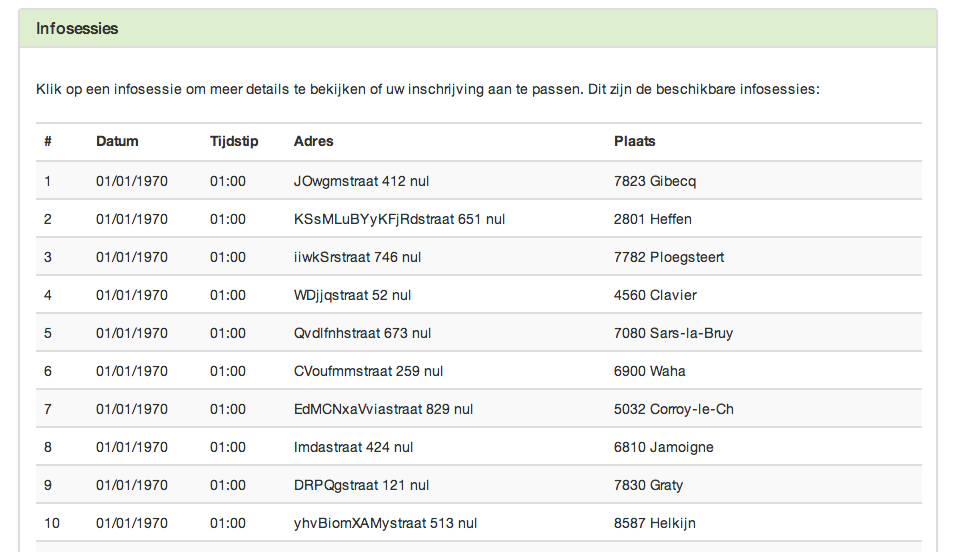
\includegraphics[scale=0.75]{img/infosessies} \\
Deze pagina geeft een overzicht van de verschillende infosessies van D\'egage. Per infosessie kan u meteen zien wanneer en waar deze plaatsvindt. Als u dan op een bepaalde infosessie drukt, krijgt u meer details te zien. Om u te kunnen inschrijven voor zo'n infosessie is het ook noodzakelijk om op een specifieke infosessie te drukken.
\subsubsection{Details infosessies} 


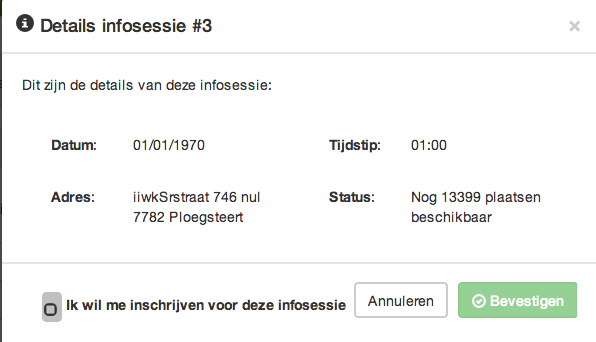
\includegraphics[scale=0.6]{img/details} \\
Zoals eerder vermeld, worden hier de details van een bepaalde infosessie weergegeven. Indien u de checkbox onderaan aanvinkt en vervolgens op \textit{Bevestigen} drukt, verwacht D\'egage dat u aanwezig zal zijn op deze infosessie. Eens u ingeschreven bent voor een infosessie is het niet meer mogelijk u in te schrijven voor een andere. Wilt u u toch inschrijven voor een andere, dan is het noodzakelijk uw huidige inschrijving eerst te annuleren.
\subsubsection{Thuisscherm}
Het thuisscherm verkrijgt u door op het logo van D\'egage te drukken, hetwelke gesitueerd is in de menubalk. Eens u ingeschreven bent voor een bepaalde infosessie, zou deze pagina er ongeveer als volgt moeten uitzien. \\
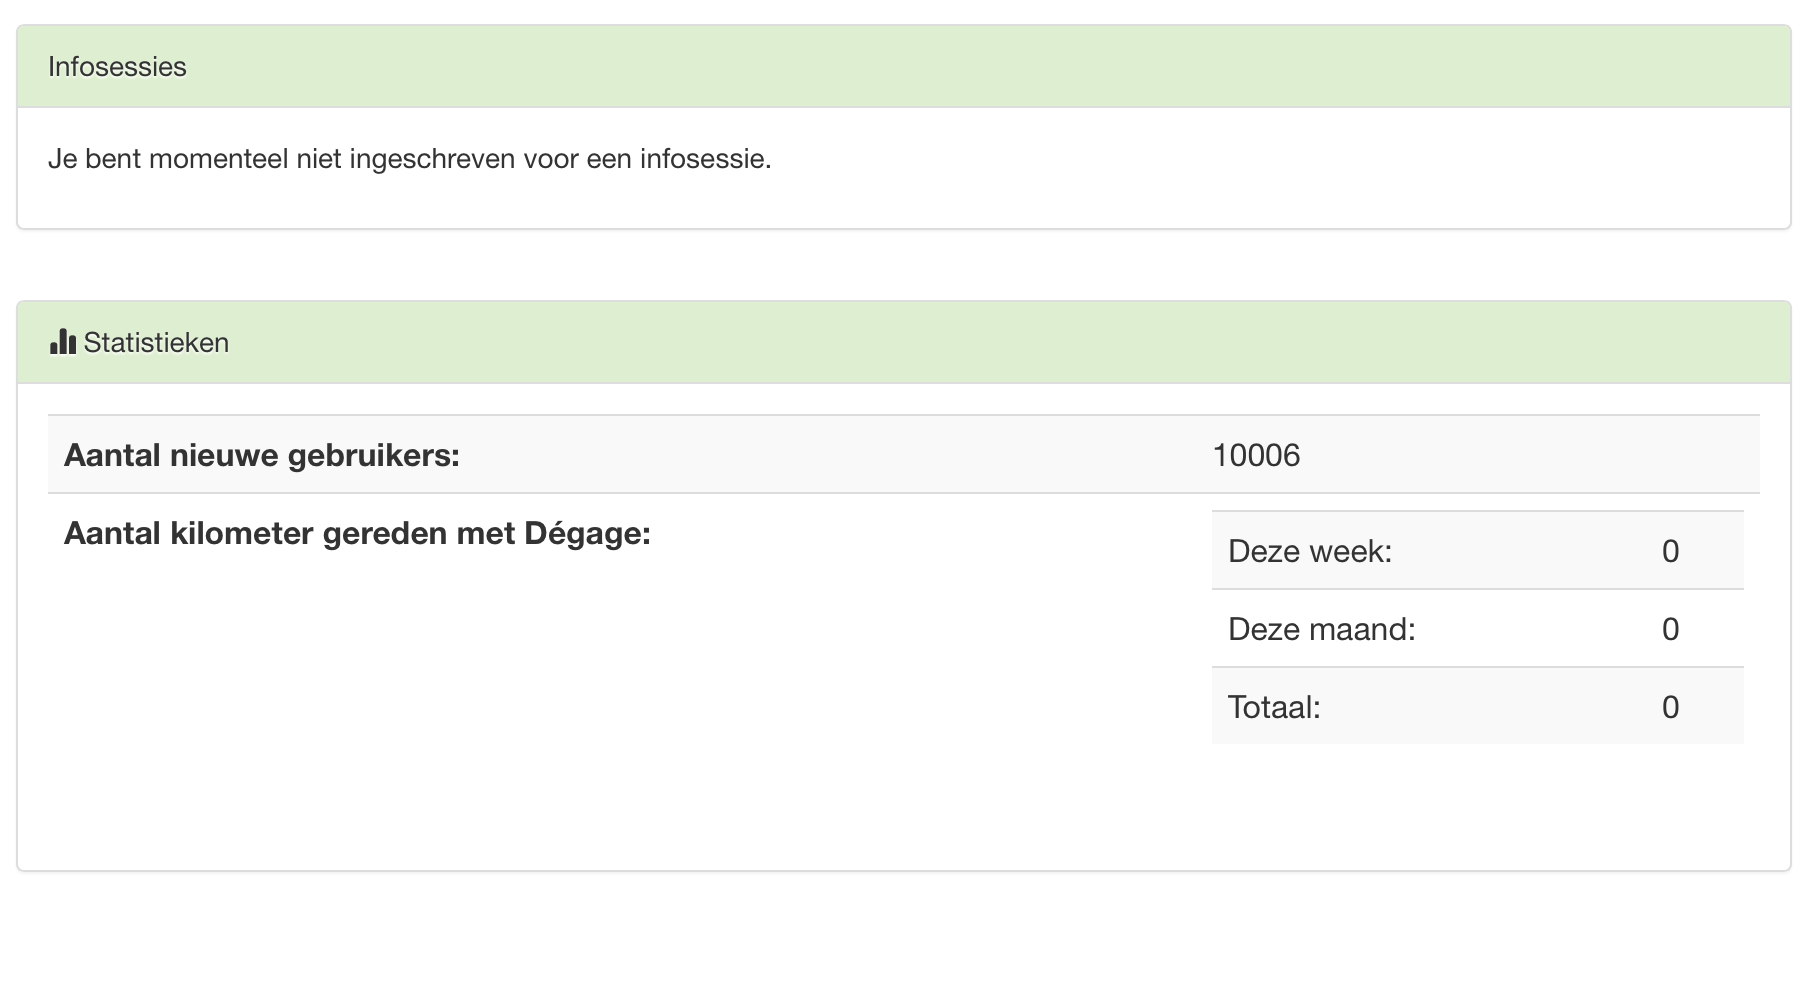
\includegraphics[scale=0.3]{img/home-autolener} \\
Hier is het mogelijk uw inschrijving te annuleren. Dit doet u simpelweg door eerst en vooral op de infosessie te drukken. Andermaal verschijnen nu de details van de infosessie. Indien u nu ditmaal de checkbox aanvinkt en op bevestigen drukt, zal de huidige inschrijving ongedaan gemaakt worden en wordt het bijgevolg mogelijk om in te schrijven voor een andere infosessie.



\subsection{Auto-eigenaar}
Indien u ook van plan bent om uw eigen auto ter beschikking te stellen van D\'egage, dan is het nodig om deze eerst toe te voegen. \\\\

\includegraphics[scale=0.4]{img/menu-autotoevoegen} \\\\
\subsubsection{Auto toevoegen}
In een normaal geval zou u het volgende moeten zien:\\\\
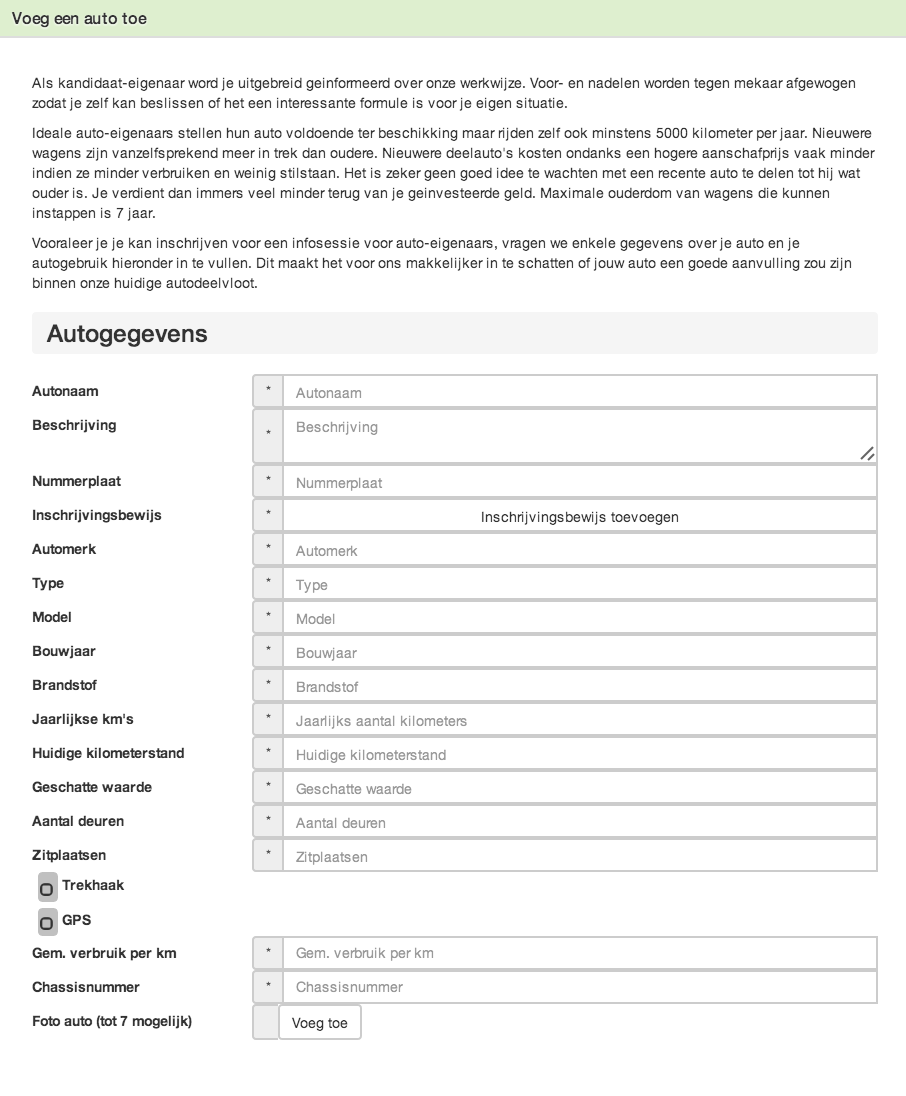
\includegraphics[scale=0.6]{img/autotoevoegen} \\

Op dit formulier is het dus nodig om allerlei gegevens in te vullen over uw auto. Het is zelfs mogelijk om foto's van uw auto toe te voegen. Indien u denkt dat alles correct is ingevuld, druk dan op \textit{Voeg auto toe} helemaal onderaan de pagina.
\subsubsection{Infosessies}
Ook indien u een auto-eigenaar bent, is een infosessie bijwonen een vereiste. Bijgevolg vragen wij u om ook in dit geval  in te schrijven voor een infosessie. Eens u een auto toegevoegd hebt, zullen wij hier echter wel rekening mee houden en u enkel de mogelijkheid bieden in te schrijven voor een infosessie specifiek voor auto-eigenaars.

\subsubsection{Thuisscherm}
Het thuisscherm verkrijgt u door op het logo van D\'egage te drukken, hetwelke gesitueerd is in de menubalk. Als u nog niet ingeschreven bent voor een infosessie, zou deze pagina er ongeveer als volgt moeten uitzien.  \\
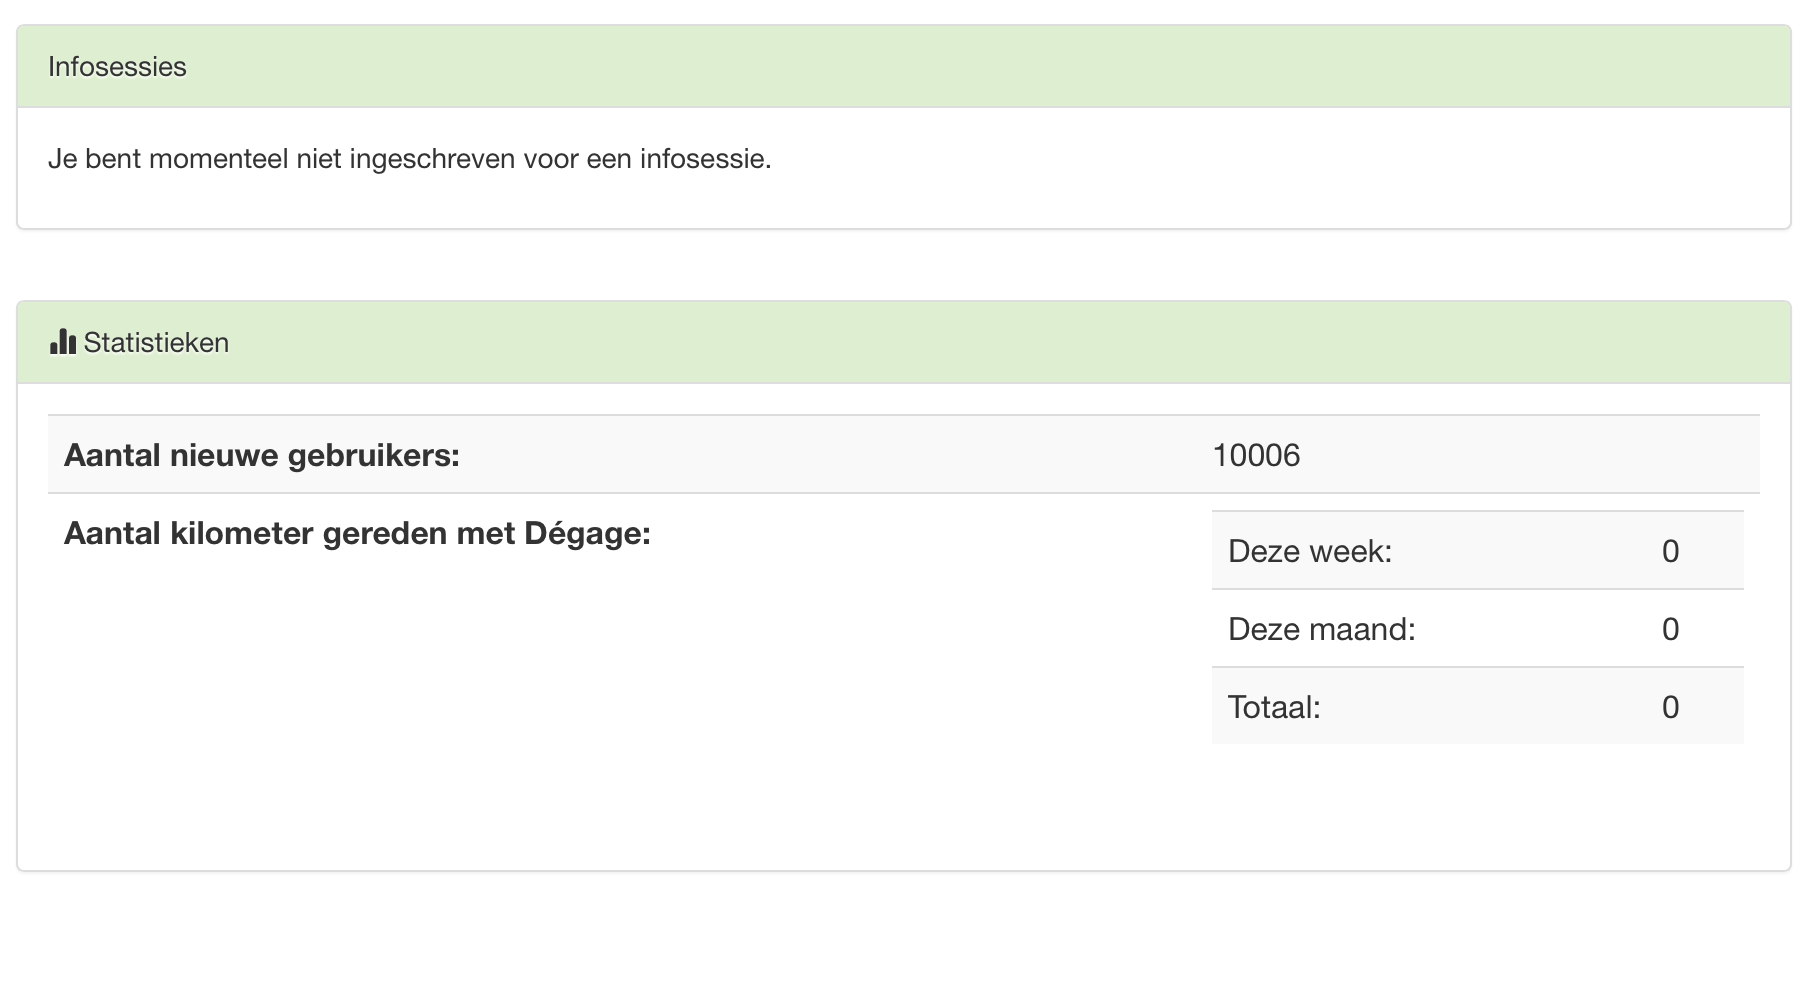
\includegraphics[scale=0.5]{img/home-autolener} \\
Onderaan zijn enkele statistieken weergegeven die handig zijn om te weten.
Als u w\'el ingeschreven bent, is het hier tevens mogelijk uw inschrijving te annuleren. Dit doet u simpelweg door eerst en vooral op de infosessie te drukken (de infosessie waarvoor u ingeschreven bent zal dan onder \textbf{Infosessies} komen). Andermaal verschijnen nu de details van de infosessie. Indien u nu ditmaal de checkbox aanvinkt en op bevestigen drukt, zal de huidige inschrijving ongedaan gemaakt worden en wordt het bijgevolg mogelijk om  in te schrijven voor een andere infosessie.
\subsubsection{Mijn gegevens}
\label{mijngegevens}
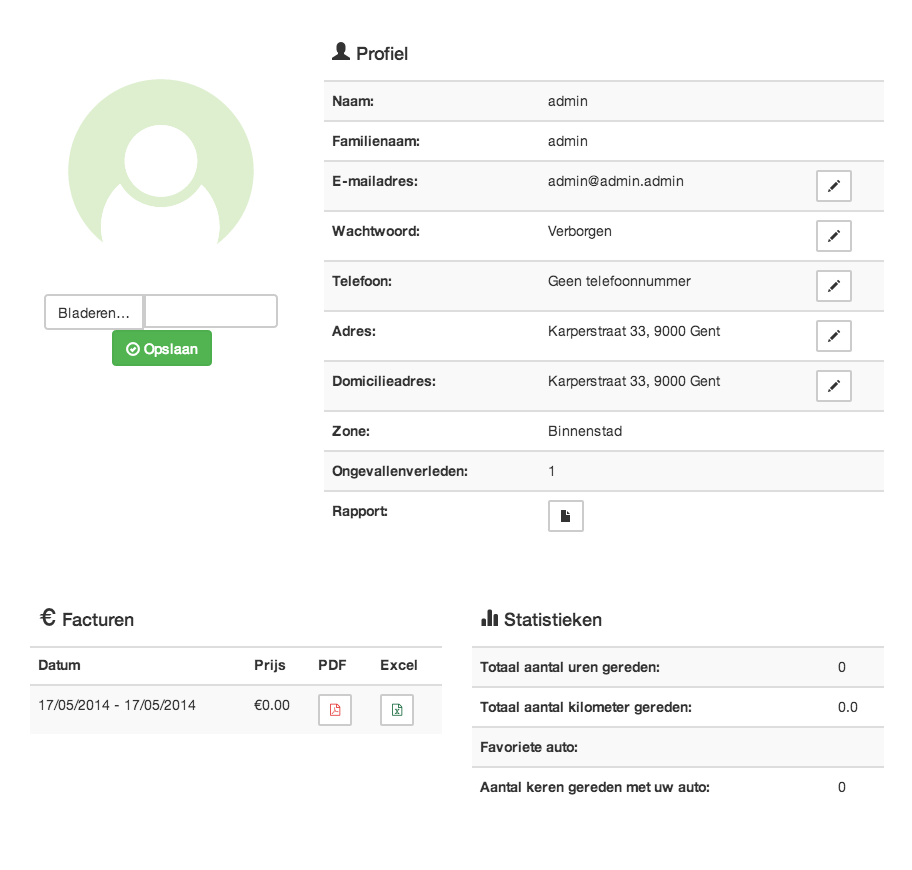
\includegraphics[scale=0.9]{mijngegevens} \\
Op deze pagina vindt u een compleet overzicht van uw eigen gegevens. Het is tevens mogelijk om een profielfoto in te stellen, welke dan telkens zal weergegeven worden hier. Onder \textbf{\euro{} Facturen} is het mogelijk om een factuur te verkrijgen zowel in \textbf{PDF} als \textbf{Excel}.
\subsubsection{Notificaties}
\label{notificaties}
In dit scherm worden belangrijke mededelingen weergegeven. Als u zich afvraagt of u belangrijke zaken gemist heeft, is het aangeraden hier eens een kijkje te nemen.







\section{Bijna lid}
Als u bijna lid bent van D\'egage, dan zal er op het thuisscherm een formulier verschijnen met al uw gegevens. Indien er nog gegevens zijn die we niet van u hebben, dan vragen wij u om deze hier in te vullen. Nu is het wachten tot een administrator alles goed keurt. Indien dit gebeurt, dan kan u de website eindelijk beginnen gebruiken.





\section{Gebruik website}
Als u al het voorgaande hebt doorlopen, bent u in het bezit van een account bij D\'egage en kan u dus eindelijk echt beginnen genieten van onze vernieuwde website. Afhankelijk of u bent ingeschreven als autolener, auto-eigenaar of administrator bent, ziet u een andere website.
\subsection{Als autolener}
Als autolener is uw eerste en enige zorg uiteraard het lenen van een auto. Beginnen doet u door op \textit{Lenen} te drukken in de menubalk.
\subsubsection{Lenen}
\label{lenen}

{\large{\textbf{Reserveren}}} \\\\
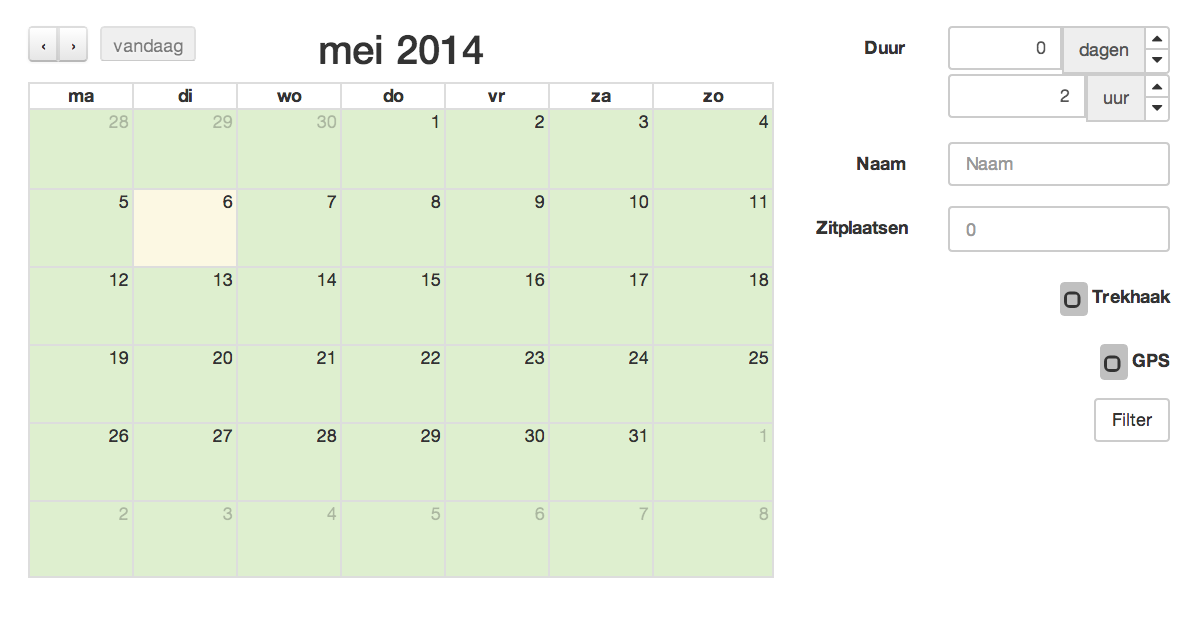
\includegraphics[scale=0.75]{img/kalender}
Vervolgens verschijnt in het groot de kalender.
\begin{itemize}
\item Lenen voor 1 dag: \\\\
Het is hiervoor voldoende een dag vanop de kalender aan te klikken.
\item Lenen voor meerdere dagen: \\\\
Om meerdere dagen te selecteren, is het nodig van de gewenste begindatum naar de gewenste einddatum te slepen (zie ook beschrijving bovenaan deze pagina).
\end{itemize}
Vooraf kan ook gebruik gemaakt worden van de filters die zich rechts van de kalender bevinden. Na het geselecteerd te hebben van de gewenste periode, krijgt u het volgende te zien:
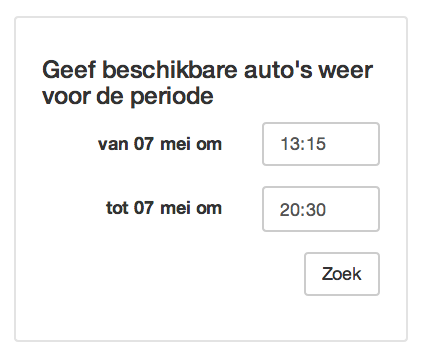
\includegraphics[scale=0.75]{img/zoeken} \\
Nu is het mogelijk de exacte uren op te geven. Vervolgens drukt u op \textit{Zoek} en krijgt u een lijst van de auto's die aan uw zoekcriteria voldoen. \\
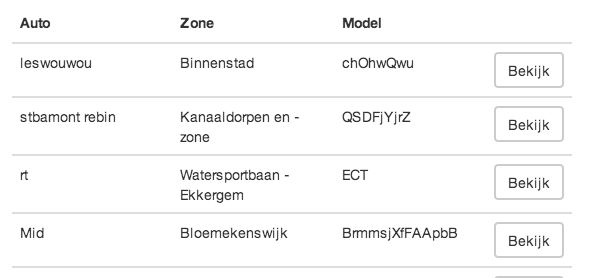
\includegraphics[scale=0.75]{img/lijstautos} \\\\
Om meer informatie over deze auto te weten te komen, drukt u eenvoudigweg op \textit{Bekijk} of gewoon op de geselecteerde rij.
\begin{center}
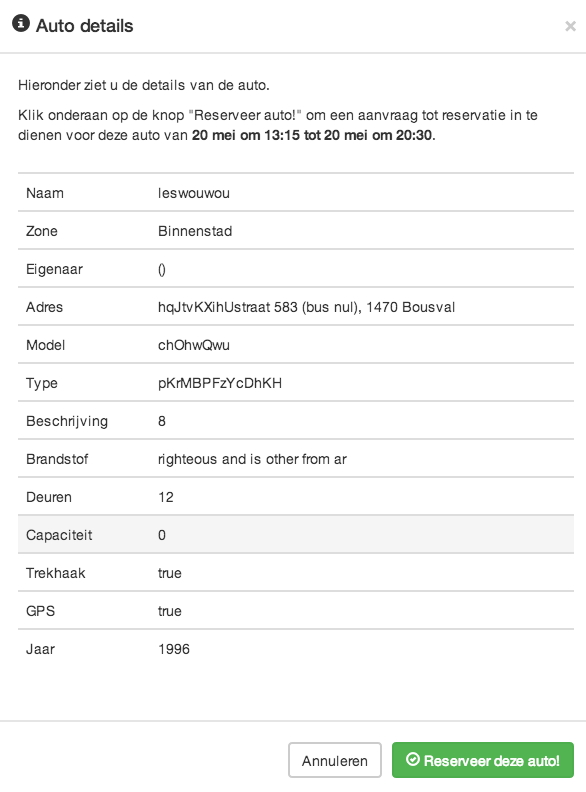
\includegraphics[scale=0.75]{img/bekijk}
\end{center}
De laatste stap is nu op \textit{Reserveer deze auto!}  drukken. Proficiat u hebt nu een auto gereserveerd voor de opgegeven periode. Indien u toch niet overtuigd bent van de auto, dan is er nog altijd een uitweg: \textit{Annuleren}. \\\\
{\large{\textbf{Ritgegevens}}} \\\\
Na een rit is het vereist al uw ritgegevens in te vullen. Dit kan enerzijds manueel, anderzijds op basis van een eerdere reservatie. Eens een rit is toegevoegd, is het vereist de kilometerstand up te daten. Dit kan door op het onderlijnde getal te drukken (hier 0) voor km. \\\\
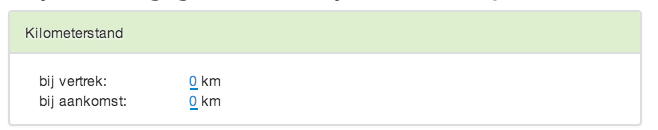
\includegraphics[scale=0.75]{img/kilometerstand}

Indien u getankt hebt, kan hier een bewijs van toegevoegd worden: \\\\
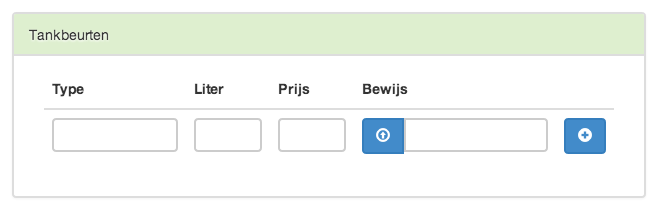
\includegraphics[scale=0.75]{img/tank} \\\\
Bij \textbf{Bewijs} verwachten we een foto of document betreffende de tankbeurt. 
\\\\
Ook schadegevallen kunnen toegevoegd worden: \\\\
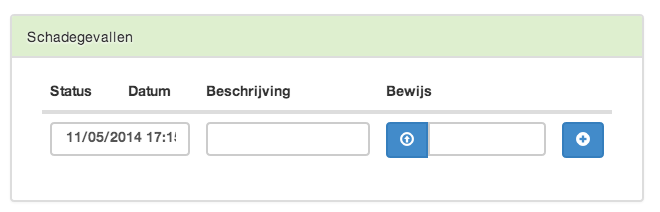
\includegraphics[scale=0.75]{img/schadegevallen} \\\\

{\large{\textbf{Mijn reservaties}}} \\\\
Hier staat een overzicht van de reservaties in behandeling enerzijds en een overzicht van de reservaties die afgelopen zijn anderzijds. \\\\
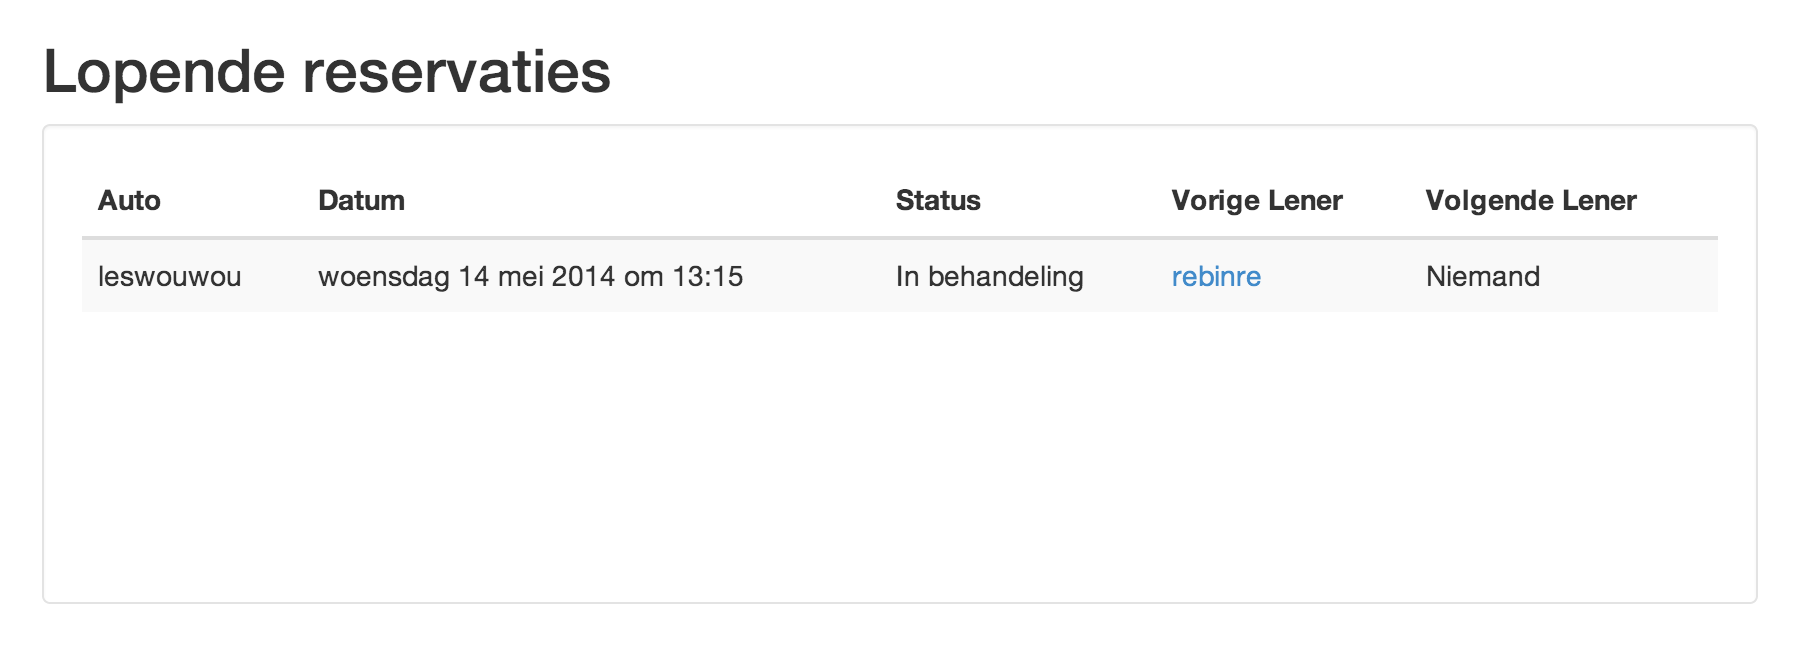
\includegraphics[scale=0.5]{img/lopende} \\\\

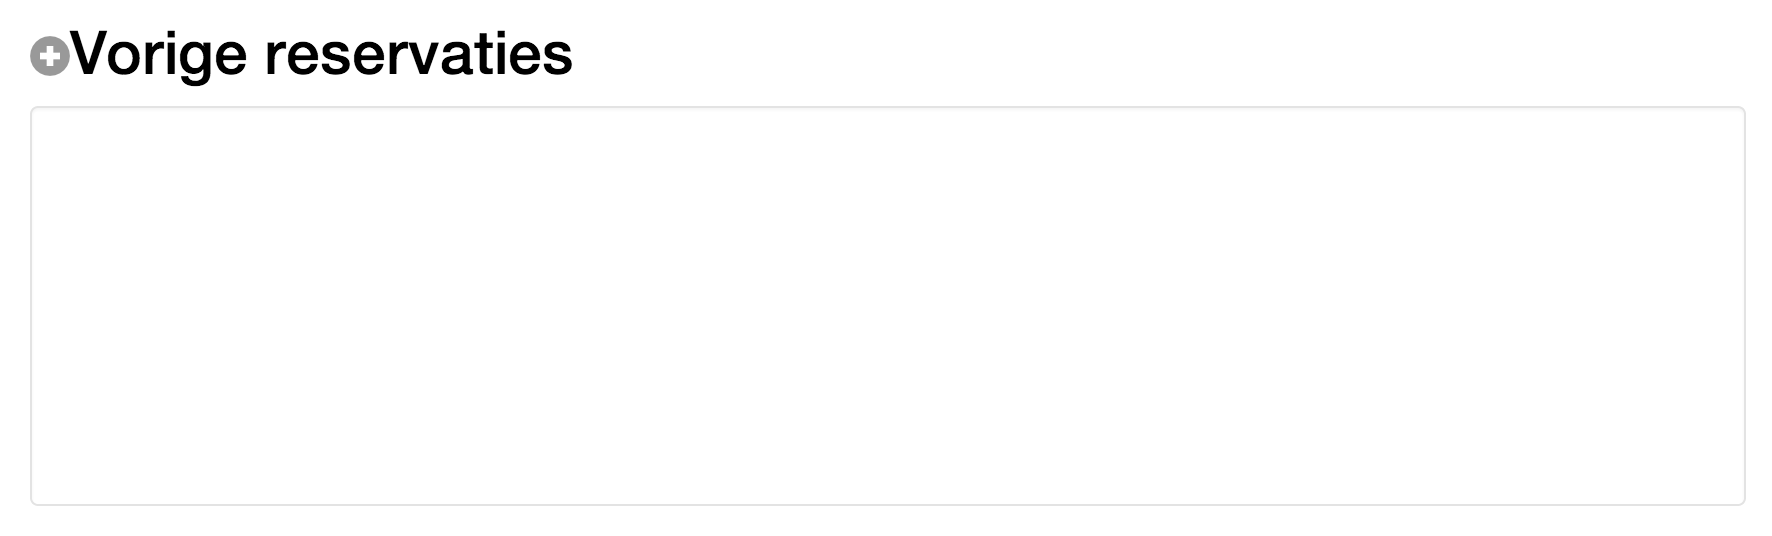
\includegraphics[scale=0.5]{img/vorige} \\\\
\subsubsection{Mijn gegevens}
Op deze pagina is het mogelijk uw gegevens nog eens na te kijken. Indien hier fouten zijn, kan u deze hier alsnog eenvoudig aanpassen. Zie ook \ref{mijngegevens}.
\subsubsection{Notificaties}
Zie \ref{notificaties}.

\subsection{Als administrator}
\subsubsection{Infosessies}
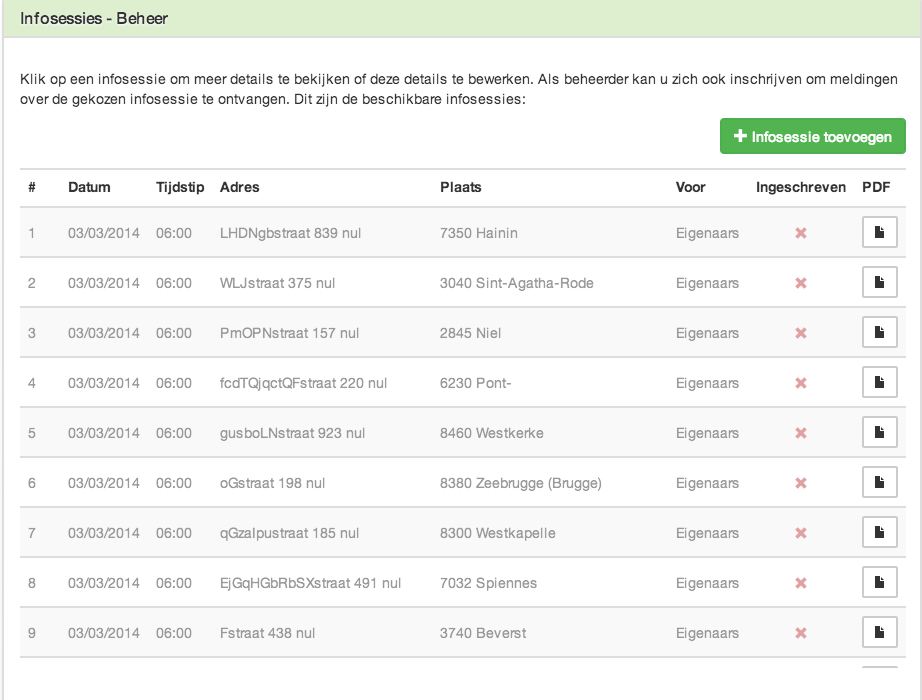
\includegraphics[scale=0.75]{img/infosessiesbeheer} \\\\
Als administrator is het natuurlijk vereist om nieuwe infosessies toe te voegen. Dit kan hier gedaan worden. Logischerwijze moet je dan op de knop \textit{Infosessie toevoegen} drukken welke zich bovenaan rechts de tabel bevindt. \\\\
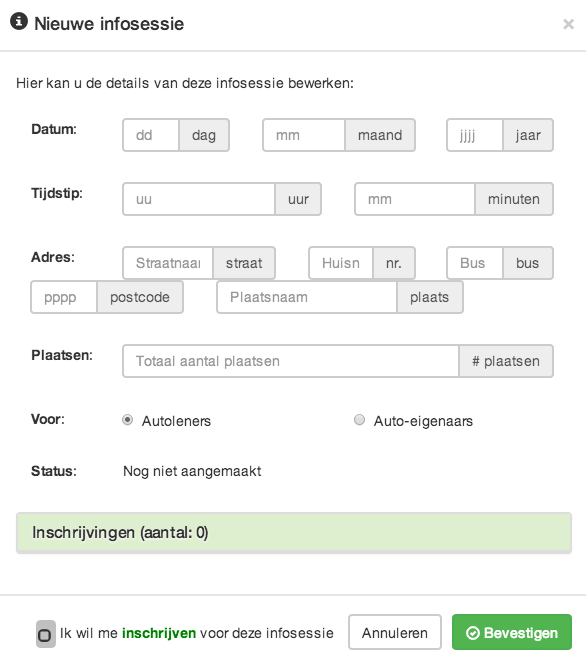
\includegraphics[scale=0.75]{img/nieuweinfosessie} \\\\
Naast de datum, tijd en plaats moet ook opgegeven worden of deze infosessie voor autoleners of voor auto-eigenaars bedoeld is, dit is toch een fundamenteel verschil. Het aantal beschikbare plaatsen van de infosessie moet verder ook vermeld worden. Ook is het mogelijk u meteen in te schrijven voor deze infosessie. Dit kan door de checkbox \textit{Ik wil me inschrijven voor deze infosessie} aan te vinken en vervolgens - na het invullen van de vereiste gegevens - op \textit{Bevestigen} te drukken. \\\\
Een bestaande infosessie wijzigen, kan door gewoon ergens in de rij van de infosessie naar keuze te drukken. Volgend scherm zal verschijnen: \\\\
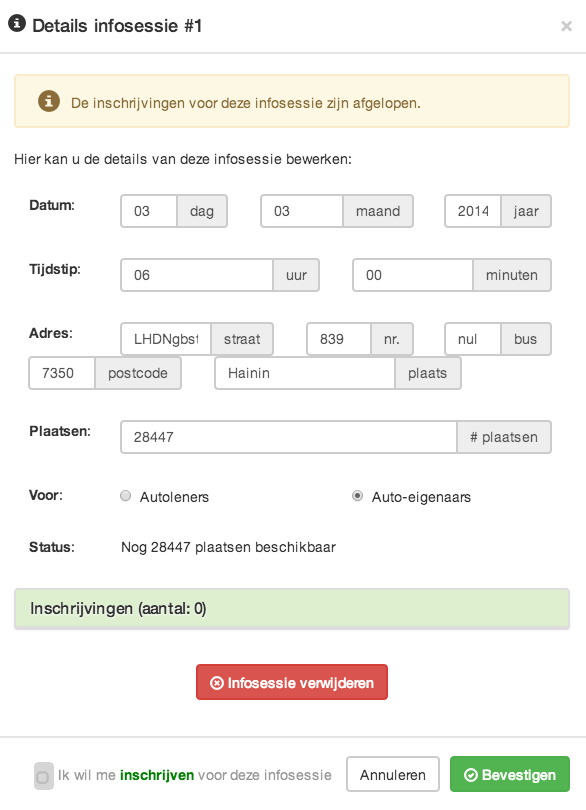
\includegraphics[scale=0.75]{img/detailsinfosessie} \\\\
Dit lijkt bijzonder goed op het scherm dat verscheen bij het toevoegen van een nieuwe infosessie. Belangrijkste uitzondering is nu dat de infosessie verwijderd kan worden - wat uiteraard niet kon bij een nieuwe infosessie. Verder wordt er een lijst weergegeven van de mensen die ingeschreven zijn voor deze infosessie.


\subsubsection{Autobeheer}
\label{autobeheer}
Deze pagina bestaat uit 4 tabbladen: \\\\
{\large{\textbf{Reservaties}}} \\\\
Het tabblad \textit{Reservaties} is nog eens onderverdeeld in 3 rubriekjes: \\
\begin{enumerate}
\item Reservatieaanvragen \\\\
Een reservatieaanvraag is  een verzoek van iemand om uw auto voor de opgegeven periode te lenen. Dit verzoek wacht dus op een reactie van de eigenaar van deze auto.
De eigenaar kan - indien het hem belieft - het verzoek goedkeuren of - indien het hem niet uitkomt - het verzoek afwijzen en eventueel vermelden waarom hij het verzoek niet accepteert.
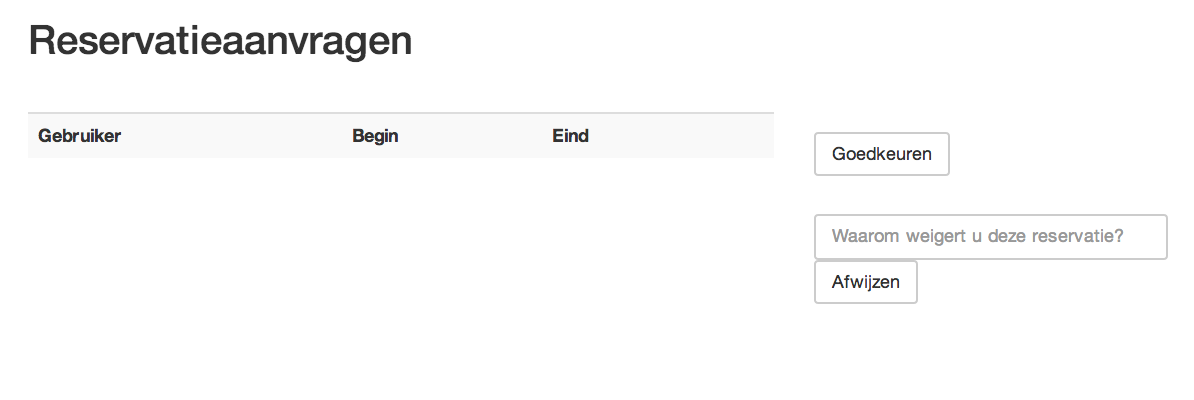
\includegraphics[scale=0.75]{img/reservatieaanvragen}
\item Geaccepteerde reservaties \\\\
Hier staat een overzicht van de reservaties die u in het verleden hebt goedgekeurd. Indien om een of andere reden u toch onmogelijk uw auto nog kan uitlenen op dat moment, is het alsnog mogelijk de reservatie af te wijzen.
\begin{center}
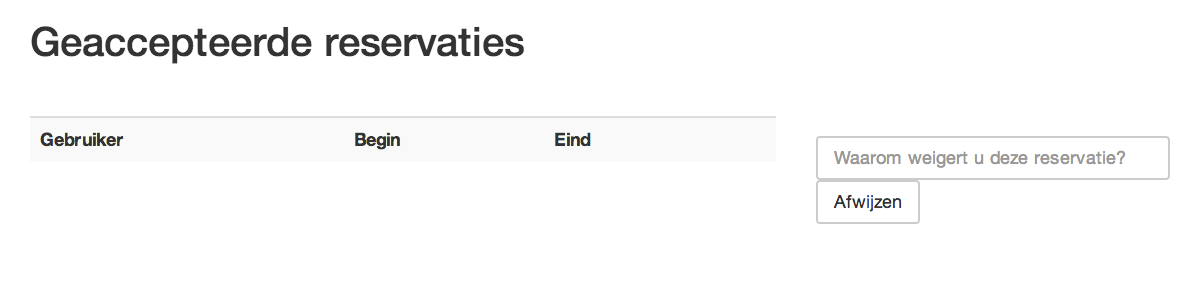
\includegraphics[scale=0.75]{img/geaccepteerd}
\end{center}
\item Afgewezen reservaties \\\\
Hetzelfde principe geldt bij \textit{Afgewezen reservaties}. Ook hier is het mogelijk om de status van de reservatie alsnog te wijzigen. In dit geval dus alsnog goedkeuren in plaats van af te wijzen.
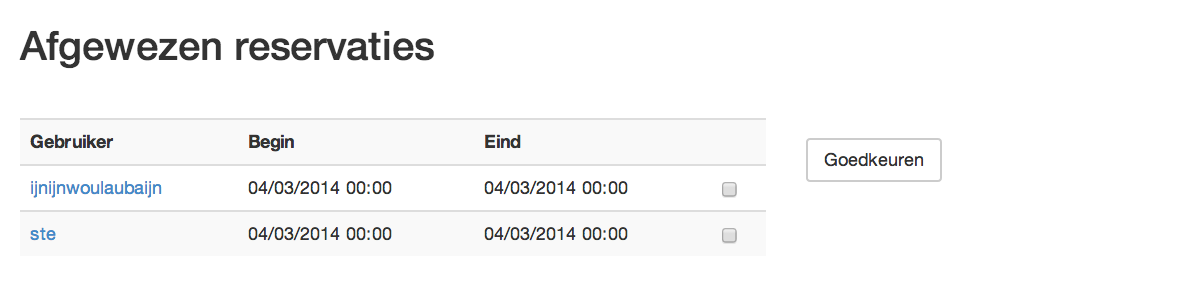
\includegraphics[scale=0.75]{img/afgewezen}
\end{enumerate}

{\large{\textbf{Ritgegevens}}} \\\\
Nadat er een rit met uw auto gemaakt is, zullen er gegevens van de rit en uw auto doorgegeven worden door de persoon die uw auto in leen had. Deze komen terecht in \textbf{Doorgegeven ritgegevens}. \\\\


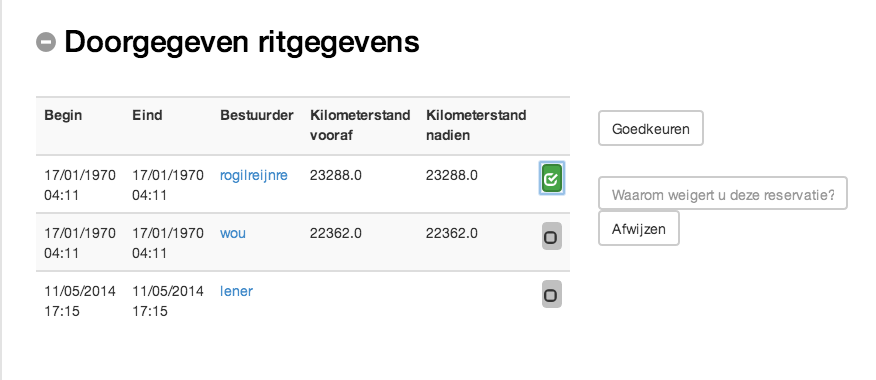
\includegraphics[scale=0.75]{img/doorgegevenritgegevens} \\\\
Nu is het mogelijk deze gegevens goed te keuren - indien u overtuigd bent van de echtheid hiervan - of af te wijzen - indien u toch uw twijfels hebt. Deze komen dan respectievelijk in \textbf{Geaccepteerde ritgegevens} en \textbf{Afgewezen ritgegevens}. \\\\

\includegraphics[scale=0.75]{img/geaccepteerderitgegevens} \\\\

\includegraphics[scale=0.75]{img/afgewezenritgegevens} \\\\
Door op het plusje te drukken links van de titel, worden deze gegevens uitgeklapt.\\\\

{\large{\textbf{Mijn auto}}} \\\\
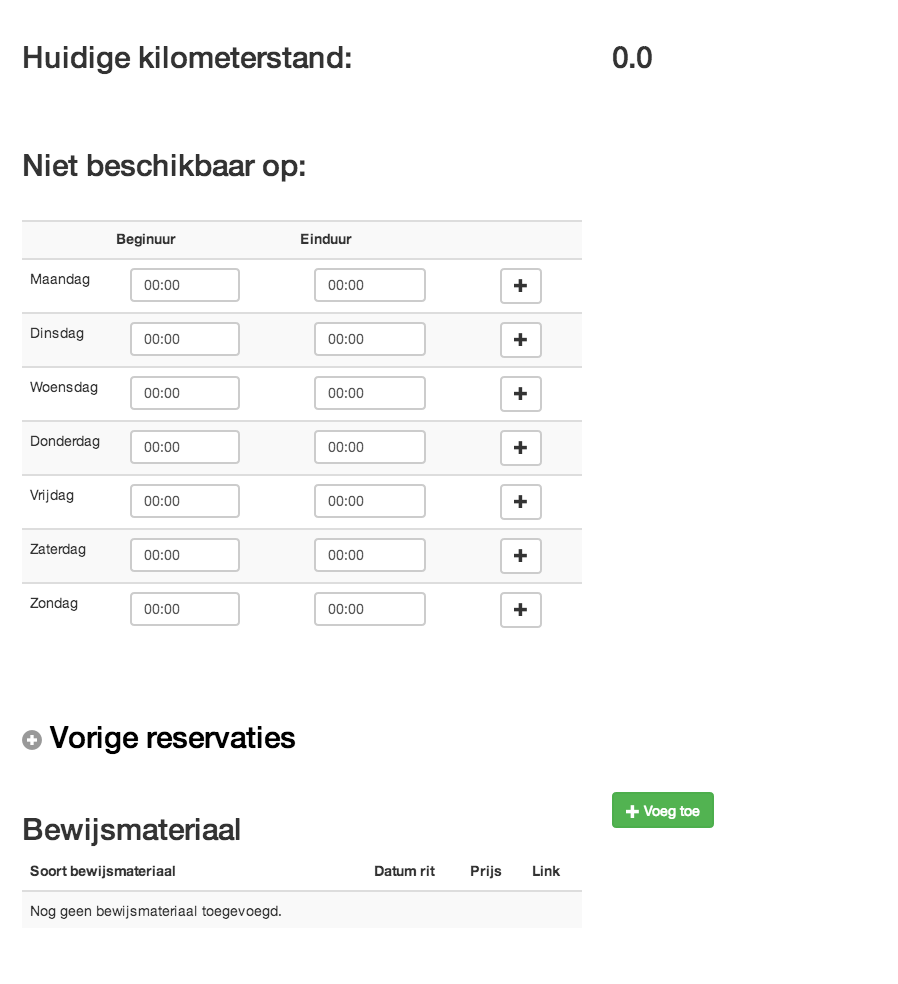
\includegraphics[scale=0.75]{img/mijnauto} \\\\
Op dit tabblad kan u eerst en vooral de kilometerstand waarnemen van uw auto.
Vervolgens kan u voor elke dag aanduiden welke uren u uw auto absoluut nodig heeft.  Om een begin- en einduur toe te voegen is het nodig om op het plusje te drukken. \\\\
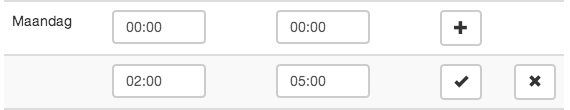
\includegraphics{reservatierangetoegevoegd} \\\\
Bij bovenstaande afbeelding is bijvoorbeeld de auto niet beschikbaar van 2u tot 5u 's morgens op maandag. Om dit te verwijderen, drukt u gewoon op het kruisje. Wilt u het begin-of einduur aanpassen? Geen probleem! Wijzig gewoon de tijd en druk vervolgens op het vinkje. Op die manier zal de reservatierange aangepast worden.

Verder wordt een overzicht van de \textbf{Vorige reservaties} opgelijst. Indien u nieuw bewijsmateriaal wenst toe te voegen, druk dan gewoon op \textit{Voeg toe} bij \textbf{Bewijsmateriaal}. \\\\
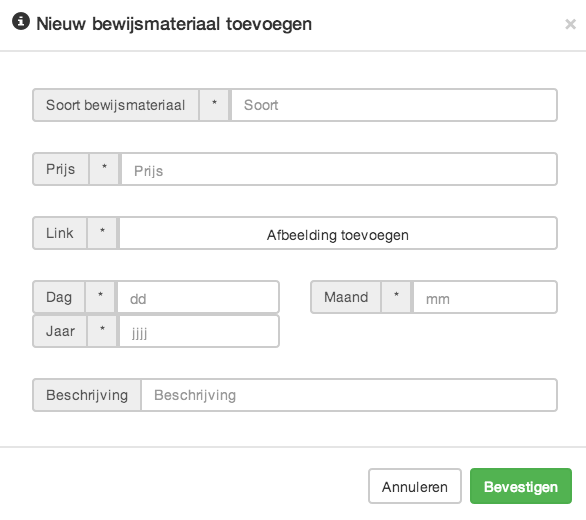
\includegraphics[scale=0.75]{img/nieuwbewijsmateriaaltoevoegen} \\\\
Vervolgens verschijnt bovenstaand venster. Enkel de beschrijving van het bewijsmateriaal is optioneel, de rest is verplicht in te vullen en deze velden zullen dus ingevuld moeten worden alvorens het bewijsmateriaal succesvol zal toegevoegd worden. Indien er fouten opgetreden zijn, zal er feedback gegeven worden over wat u precies fout hebt gedaan.

{\large{\textbf{Schadegevallen}}} \\\\
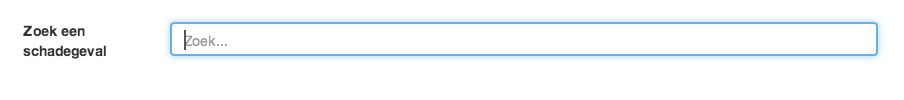
\includegraphics{zoekeenschadegeval}
Hier is het mogelijk om een bepaald schadegeval op te zoeken.
\subsubsection{Lenen}
Zie \ref{lenen}.
\subsubsection{Beheer}


{\large{\textbf{Gebruikers}}} \\\\
Op deze pagina is het mogelijk om de rollen van gebruikers te wijzigen en om een registratie van een gebruiker definitief goed te keuren.

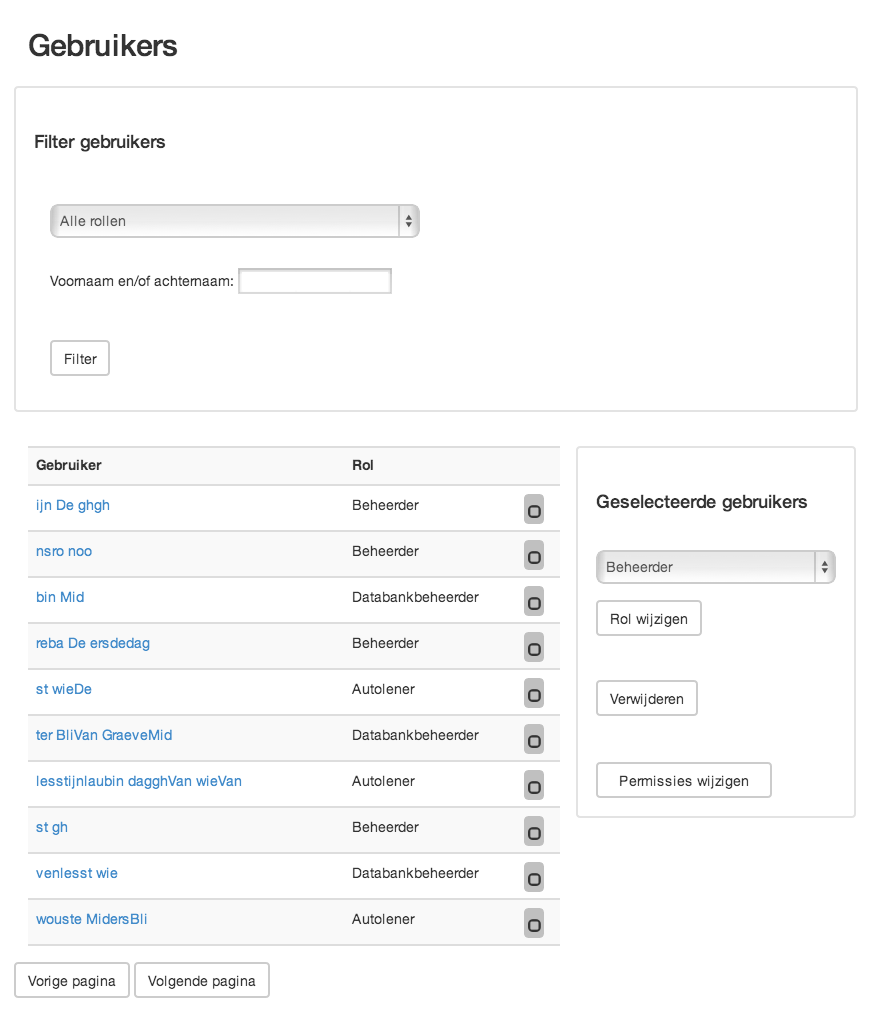
\includegraphics[scale=0.6]{rolgebruikerwijzigen} \\
Dit stuk is bedoeld om de rol van een gebruiker te wijzigen. Aanvankelijk kan u de gebruikers filteren op basis van een rol enerzijds of op basis van een naam anderzijds. Vervolgens verschijnen in de tabel alle gebruikers die voldoen aan het zoekcriterium of gewoonweg alle gebruikers indien geen criterium opgegeven is. Via de knoppen \textit{Vorige pagina} en \textit{Volgende pagina} kan u door de gebruikers bladeren. Nu is het noodzakelijk alle gebruikers aan te vinken waarvan u de rol wilt wijzigen. Bij \textbf{Geselecteerde gebruikers} selecteert u dan de nieuwe rol van de geselecteerde gebruikers en drukt u op \textit{Rol wijzigen}. De geselecteerde gebruikers kunnen ook verwijderd worden via \textit{Verwijderen}. Via \textit{Permissies wijzigen} is het zelfs mogelijk om voor elke gebruiker volledig in te stellen wat deze wel en/of niet mag doen. Dit gaat van infosessies aanmaken tot gebruikers verwijderen. \\
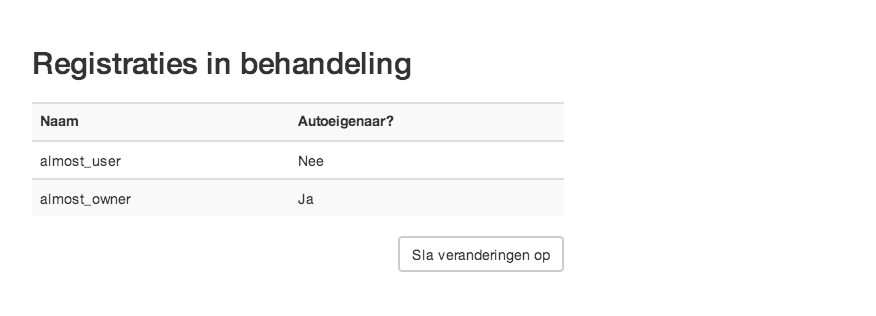
\includegraphics[scale=0.6]{registratiesinbehandeling} \\
Via \textbf{Registraties in behandeling} is het mogelijk om de registratieprocedure van een gebruiker eindelijk volledig af te ronden. Als u op een naam drukt, wordt het volgende bekomen:

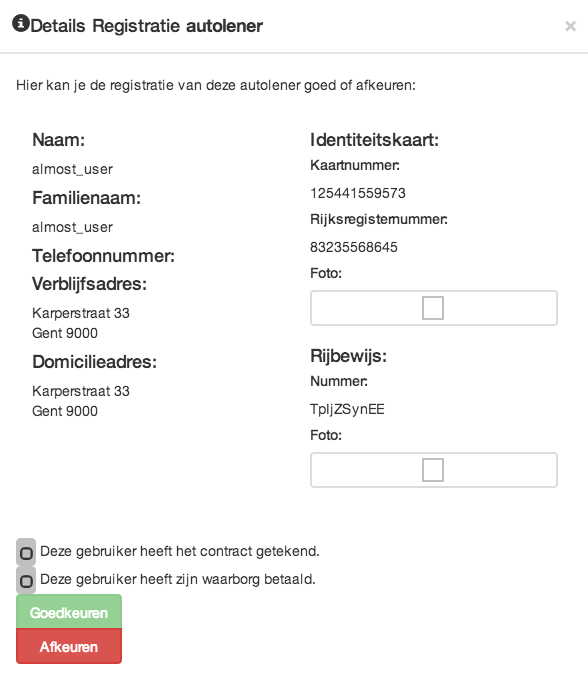
\includegraphics[scale=0.5]{detailsregistratieautolener} \\
Hier wordt nog eens alle informatie van de gebruiker weergegeven.
Door de checkboxen \textit{Deze gebruiker heeft het contract getekend.} en \textit{Deze gebruiker heeft zijn waarborg betaald.} aan te vinken en dan op \textit{Goedkeuren} te drukken, wordt de gebruiker definitief lid en moeten geen stappen meer ondernomen worden door de gebruiker. Hij is nu eindelijk volwaardig lid van het systeem.

{\large{\textbf{Beheer auto's}}} \\\\
Auto's die toegevoegd worden, moeten gekeurd worden door administrators. Dit kan hier gebeuren. Als alles goed gaat, wordt een lijst met alle nog goed te keuren auto's weergegeven hier. Door op de rij van de auto in de tabel te drukken, worden meer details getoond. Onderaan \textbf{Details auto} is het dan mogelijk de auto te accepteren of te weigeren. Als de auto goedgekeurd wordt, zal de eigenaar van de auto een notificatie krijgen.\\\\
{\large{\textbf{E-mail voorkeuren}}} \\\\
Voor een aantal gebeurtenissen stuurt D\'egage emails naar zijn gebruikers. Voor elke gebeurtenis is het hier mogelijk om de tekst en opmaak van de emails te wijzigen. Er kan hier ook beslist worden om voor een bepaalde gebeurtenis geen mails meer te verzenden. \\
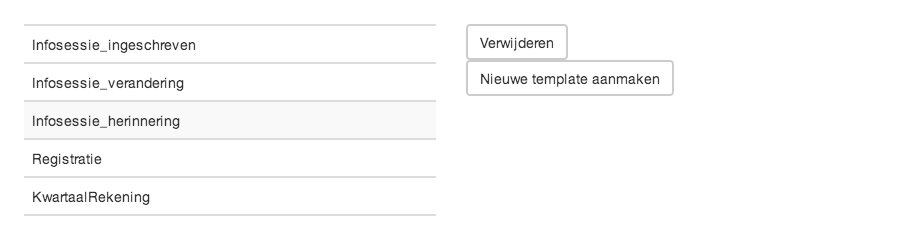
\includegraphics{overzichttemplates}
Bovenaan zijn de gebeurtenissen vermeld voor het versturen van mails. Er worden mails verstuurd voor de volgende gebeurtenissen:
\begin{itemize}
\item een gebruiker heeft zich succesvol ingeschreven voor een infosessie
\item er is iets veranderd aan een infosessie (bijvoorbeeld ander aanvangsuur)
\item er vindt zeer snel een infosessie plaats waarvoor een gebruiker is ingeschreven
\item een gebruiker heeft zich succesvol geregistreerd
\item er is een kwartaal verstreken en bijgevolg zal een nieuwe rekening beschikbaar zijn
\end{itemize}
Als u nu op een bepaalde gebeurtenis drukt, zal het onderdeel \textbf{Template wijzigen} zich aanpassen. \\
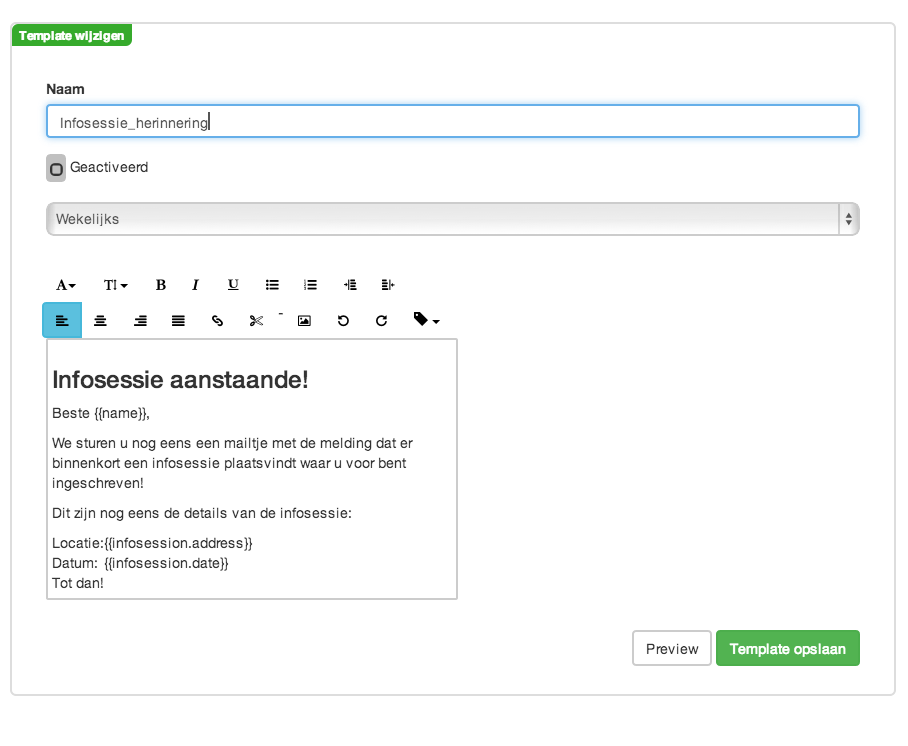
\includegraphics{templatemails} \\
Het is hier mogelijk om de naam te wijzigen, deze gebeurtenis voor het versturen van emails te (des)activeren en de tekst van de mail te wijzigen. Na de aanpassingen doorgevoerd te hebben, vergeet dan niet op \textit{Template opslaan} te drukken. Via \textit{Preview} is het mogelijk de mail in de ogen van de gebruiker te zien.
\\\\
{\large{\textbf{Bewijsmateriaal}}} \\\\
Hier is het mogelijk bewijsstukken en tankbewijzen te accepteren/weigeren. \\\\
{\large{\textbf{Prijsintervallen}}} \\\\
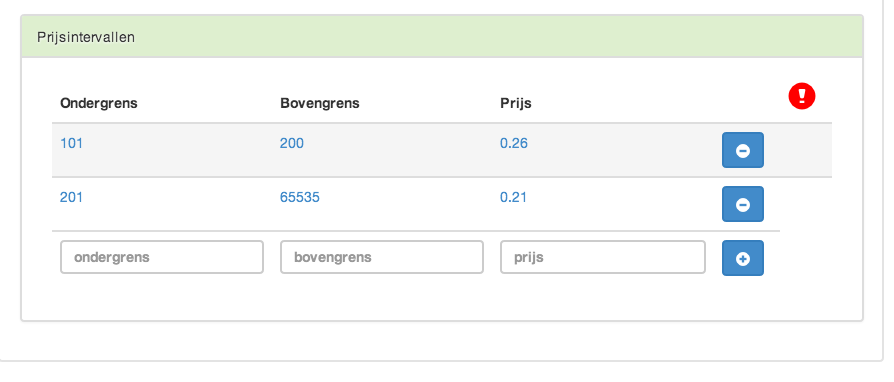
\includegraphics{prijsintervallen}\\
Hier is het dus mogelijk om de prijsintervallen in te stellen. Bovenstaand voorbeeld duidt erop dat tussen 101 km en 200 km de prijs per km 26 cent bedraagt en die tussen 201 en 65535 21 cent. Het is ook eenvoudig om een nieuw prijsinterval toe te voegen. Het volstaat \textit{ondergrens}, \textit{bovengrens} en \textit{prijs} in te vullen en vervolgens op het plusje te drukken. Let wel de ondergrens en bovengrens moeten decimaal zijn, de prijs een kommagetal.\\\\
{\large{\textbf{Back-up databank}}} \\\\
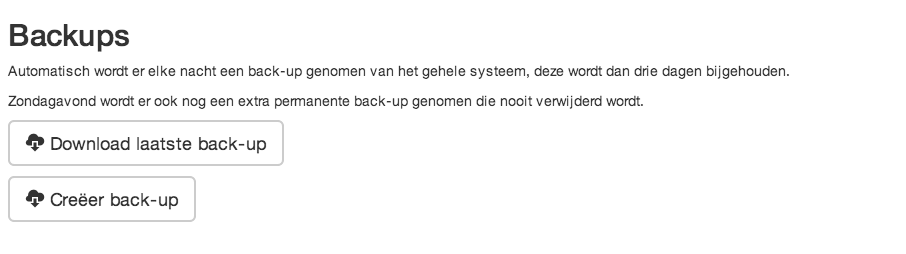
\includegraphics{backups} \\
\subsubsection{Mijn gegevens}
Zie \ref{mijngegevens}.
\subsubsection{Notificaties}
Zie \ref{notificaties}.



\subsection{Als auto-eigenaar}
\subsubsection{Autobeheer}
Zie \ref{autobeheer}.
\subsubsection{Lenen}
Zie \ref{lenen}.
\subsubsection{Mijn gegevens}
Zie \ref{mijngegevens}
\subsubsection{Notificaties}
Zie \ref{notificaties}.















\end{document}
